\chapter{Program Counter Register}

During the course of this semester, we will build a 64-bit computer so that we can understand how it works.  To do this, we will make a synthesizable machine in Verilog, a common hardware description language (HDL).  

A computer runs a program by executing individual instructions in sequential order.  The instructions are stored in memory and are accessed by their memory address.  During each clock cycle, an instruction is fetched from memory and executed on the processor.  The memory address of the next instruction to fetch is stored in a register called the Program Counter (PC).  During Lab 1, we will build and test the Program Counter register.  In Lab 2, we build an incrementer (to count to the next instruction) and a mux (to select between the incremented count or a new starting value).   

\section{Program Counter Register}

In order to make the Program Counter, we are going to make a Verilog module that explains how to build a register (a D flip-flop).  Let me unpack the previous sentence:
\begin{enumerate}
	\item Verilog is a Hardware Description Language (HDL).
	\item We write Verilog code to tell Vivado how we want our register module to behave.
	\item Vivado reads our Verilog code and synthesizes a realizable digital hardware design that meets the behavior that we specified.  Thank you Vivado!
	\item Vivado also simulates the behavior of the hardware, allowing you to test your design without building/programming hardware.
\end{enumerate}   
Consider the Verilog code in Listing~\ref{code:register}.  It is made up of three sections: a header (which has the include command), a port list or interface (which specifies the signals coming in or going out of our module), and a body or implementation (which describes how to build it).

\Verilog{Verilog code to make a register.}{code:register}{../code/1_fetch/register.v}

The first part is the header.  We will use this same header each time.  It tells the Verilog compiler to get all the data from a file called definitions.vh.  The extension vh is a Verilog header.  We use this to specify common pieces of data we will use across our design, so that all the components we build will be consistent.  By putting them in one file, we make it easier to maintain, and prevent mistakes that can happen easily by having multiple copies of these basic pieces of data.  For our first component the piece of data we will be using is WORD (set to 64), which is the size of the memory addresses our computer will use (how many bits).  Note that if we build things based around WORD, rather than the number 64, we can just change the value of WORD in the file and get a computer with a different size with a couple key strokes.

The second part is the port list or interface.  In this area we specify what signals are coming in (input), going out (output), or could go either direction (inout).  Ports can be defined as either "wire" or "reg".  This can be confusing to some students.  Think of it this way: 
\begin{enumerate}
	\item Wire
	\begin{enumerate}
		\item A wire is just a conductor that connects one component or module to another.
		\item The value on a wire can only be changed by using combinational logic.
		\item It has no memory, meaning that the value on the wire is driven by the results of combinational logic at that particular moment.
		\item Module inputs are always wires
		\item Module outputs can be wires or regs.
	\end{enumerate}
	\item Reg
	\begin{enumerate}
		\item A reg more closely resembles a variable in software programming languages.
		\item A value of a reg can only be set by using sequential logic.
		\item A reg has memory, meaning that the value of the reg will remain the same until a sequential logic element updates it.
		\item You can directly set a reg to a value using a procedural assignment.
		\item Regs can be used internally in a module (neither input nor output), or they can be used as module outputs.  They cannot be used as module inputs. 
	\end{enumerate}
\end{enumerate}

\begin{figure}
	\caption{Module Diagram.}\label{fig:modulediagram}
	\begin{center}
		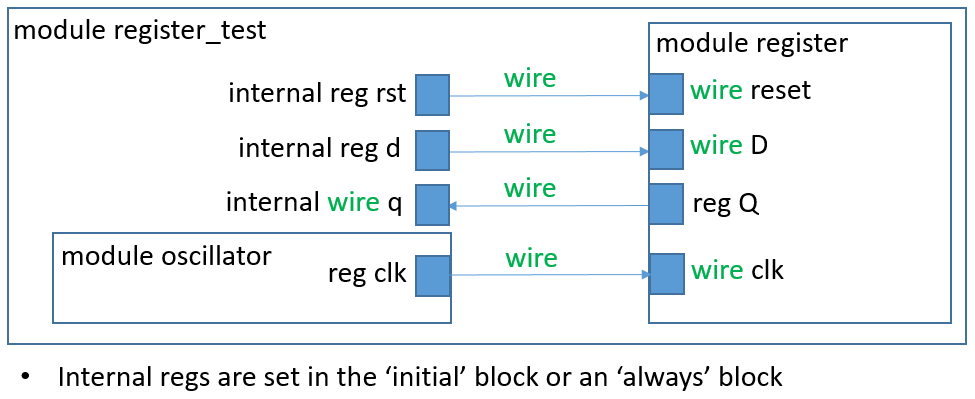
\includegraphics[width=4.75in]{../images/register_test_module_diagram.png}
	\end{center}
\end{figure}

If you don't specify anything for the port type, you will get a wire - it is the default.  In our case we have four signals: three inputs, and one output that is a register.  The first two inputs are single-bit wires.  One is the clock, which specifies the timing, and the other is reset, which clears the contents of the register (makes them zero).  The final input is the value we want to store in memory, and I have called it D, following the convention of digital logic.  D has multiple bits that are numbered from WORD-1 down to 0.  Thus the leftmost bit is 63 in this case, and the rightmost bit is 0\footnote{If you want to be technical this is called little endian, since the little end (the least significant or unit bit) is going into the first memory location (bit 0).  If you reversed the order by putting the 0 first and the WORD-1 last it would be big endian, since the big end (most significant bit) would go in the lowest addressed bit.}.  The output Q (also the digital logic conventional name) is a register (it will hold its value) and should also be of size WORD and follow the same order as the input D.

To help clarify this, please examine Figure~\ref{fig:modulediagram}, which shows the interconnection of the modules in this lab.

The final section is the body or implementation.  It is composed of a single thread of code, that will keep running (hence always).  It will run one time every time there is a positive edge (0 to 1 transition) for either the clock or reset.  Reset has higher priority, so if reset is asserted the register is cleared (Q is set to zero), otherwise the value of D is stored it Q.  That is it.  A nice, simple module.  Please note that the provided register module is fully operational.  You do not need to modify it.

\section{Testbench}

We now want to test this.  To test it, we need to tell the simulator to build a copy (instantiate) the module, and then we will need to supply the inputs and look at the outputs to verify that the module works correctly.  Consider the testbench in Listing~\ref{code:register_test}.

\Verilog{Verilog code to test a register.}{code:register_test}{../code/1_fetch/register_test.v}

Like our register it starts with our standard header, but this time there are no ports!  A testbench is providing all the signals to simulate the inputs to the unit under test (UUT) and thus does not need them.  This is how Verilog finds a top level simulation module - there are no ports.  The clock signal will be driven by a module named oscillator, which will give us a nice square wave with period CYCLE, which is another constant defined in our definitions.vh file.  The code thus makes an oscillator and a register, then runs the 'initial' section (it runs once at the start then never again).  The initial section sets the value of the inputs then waits a CYCLE.  The last couple of delays are not full cycles.  I did this for two reasons:
\begin{enumerate}
\item To show you how to make Verilog do calculations for you.
\item To remind you that the input won't necessarily be nice and perfectly timed to your register.  Unsynchronized signals happen, and is a frequent cause of problems, hence the need to test.
\end{enumerate}
This is by no means an exhaustive testbench, but run it and look at the output.  Does it do what you expect?  What else might you want to test?  Add this to your testbench and run it again to see if the register works.



\begin{figure}
\caption{Timing diagram.}\label{fig:registertiming}
\begin{center}
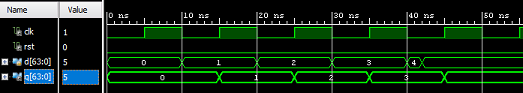
\includegraphics[width=4.75in]{../images/register_test_timing_diagram.png}
\end{center}
\end{figure}

\section{Using \LaTeX\ for Your Write-up}
This section was originally written by Dr. Schubert, so any first person references are from Dr. Schubert.

All that is left is to write it up.  I am going to have you use \LaTeX\ to do your lab reports. Note how I include files, programs, and images.  It is worth noting that \LaTeX\ will automatically make the table of contents and bibliography for you also.

Why use \LaTeX\ ?  There are lots of reasons, but here are a few that matter in this course:
\begin{enumerate}
\item It typesets programs from the actual source, no need to copy the program and have spell checkers and grammar editors mess things up.
\item It quickly and correctly handles equations.
\item It automatically handles table of contents and bibliographies.
\item It is free, and generates high quality documents (book quality) - it is open source since before open source.
\item It is used in publication of research documents.
\item It is the only large program believed to be error free in its source code, and have no missing features (development is complete!)
\end{enumerate}


\subsection{Background}

\TeX\ refers to both a language for typesetting and the program (compiler actually) that does the typesetting.  \LaTeX\ is a macro package which sits on top of \TeX\ and provides additional functionality, and has become synonymous with the language variant (dialect) of \TeX\ which it created.  Since \LaTeX\ is hugely popular and really useful, \TeX\ and \LaTeX\ have become synonymous to most people, and I will treat it so from now on.  A note on pronunciation: \TeX\ is in Greek letters - tau epsilon chi and hence is pronounced `tek' not tex (similar for \LaTeX\, which is pronounced `lay-tek' not latex).

\TeX\ is not a WYSIWYG (what you see is what you get) typesetting program like many editors you are familiar with, as it was designed to be a tagged language like the more recent html (yes, \TeX is older).  The idea is not to spend time thinking about how it should look, but rather to classify what it is and let the automated standards set the text by what the text is\footnote{For instance, note the chapter, section, and subsection commands in the tex files.  \LaTeX\ assigns a number, records it, the title, and page so it can automatically put it in the table of contents for you.}.  To provide flexibility and extension (and it was designed by one of the greatest computer scientists, Donald Knuth) it was set up as a programming language with a compiler.  Since \LaTeX\ is a programming language, we have a comment character \% that I had to escape by putting a \textbackslash before it to make it print.  Whitespace past the first space (word separation) is ignored, except for a blank line, which means start a new paragraph.  More than one blank line is ignored.  To get more space, you issue a command, such as \verb1\vspace{.25in}1, which puts a quarter inch of vertical space.  \LaTeX\ also knows pt (points), px (pixels), pc (pica), mm (millimeters), cm (centimeters), em (width of an `m'), and many more.  By default the space is not placed if it does not separate some object (i.e. at the top of a page), but you can force it by using \verb1\vspace*{.25in}1.  Starred commands are just versions of the main command.

There are many more commands than we could describe in this brief intro, including commands to let you define new commands and environments.  We will not need too many fancy commands, we only need to describe the commands to include figures, code, and equations.  If you want to learn more, then I have links to free manuals online at r2labs.org.

\subsection{Compile Process}

One thing that will help you a lot in working with \LaTeX\ is how the compile process works.  \TeX\ is a two pass compiler, but it does only one pass each time it runs.  Allow me a brief introduction to compilers, which is a great course if you can take it.

When you are compiling a file you have control statements (branches, loops, conditional execution statements like if or switch/case) that require you to know how many program lines ahead or behind something is in the assembled code, which you will not know at the start.   While you are often just putting in a flag or label to be handled by the assembler later, you in truth don't even know if they actually put the destination of the transfer of control, and thus have an error.  One easy way of handling this is to run through the process twice, collecting labels and such the first time and then doing the compile the second time through, which is what a two pass compiler does.  \TeX\ collects all the labels, notes all the chapter, section, and other structures, identifies all the bibliography references, and so on and puts them in a special auxiliary file for the next pass.  It will also create a DVI file, which has most things right, but will lack table of contents, references, bibliography, and such.  The second time through it already has the information before the file runs so it reads that first and uses it to create a fully correct output.

A logical question at this point is why not just have it run twice on its own?  Well, in the 1980's computers were small and slow, so each run of \TeX (we didn't even have \LaTeX\ at first) took an appreciable amount of time.  If you know the compile process, there are times you only have to run things once, like small spelling changes not in a title, chapter, etc.  Allowing people to do only one pass at a time was a big advantage (some \TeX\ compiles I had to do could take 10 minutes even in the 1990's).  Bibliographies are handled by an external program called BibTeX, which reads the .aux file to find the references (thus you need to run \LaTeX\ first), then pulls the data from the .bib files you specify in the calling command in your .tex file and creates a .bbl file.  The .bbl file contains all the info formatted how the bibliography should look.  \LaTeX\ reads this in the first pass and copies it over to the .aux file and resolves the links to the text references.  The next run of \LaTeX reads all this in and places both the bibliography and the cross references.  This means that to get a bibliography in you must run \LaTeX\, BibTeX, \LaTeX\, then \LaTeX\ once more.  You only need to do this if you add new reference, which in the labs will be once, provided you don't delete those intermediary files.

\subsection{Getting Started with LaTex}

Now that you have some background knowledge, we need to learn how to build a document on your computer.  There are many ways to do this, including text editors and command line tools.  I prefer using a more user-friendly editing and buidling environment.  While there are numerous options available, I choose to use TexStudio.  It is installed on all ECS computers, and it is available for free download at home.  For each lab, you will want to make a copy of LabN.tex and name it Lab1.tex, Lab2.tex, etc.  After creating Lab1.tex, I would recommend opening Lab1.tex and building it before making any changes.  Then make some changes, rebuild, and view those changes in the PDF that is generated.  Steps to build a document in TexStudio are:
\begin{enumerate}
	\item Open TexStudio on your lab computer
	\item Use the menus open Lab1.tex
	\item Click on the double green arrow icon near the top.  If you hover over it, it says "Build \& View".
	\item This should produce a PDF document on the right side of the TexStudio window
\end{enumerate}

This document should build properly as long as you don't modify it.  Once you start editing, it is possible that you will get compile errors.  These errors are listed in the bottom pane of TexStudio.  Like many compilers, they are sometimes cryptic and don't lead you directly to the problem.  The most common problem (by far) is using an underscore with using the escape character (backslash) first.  For example, look at the fetch1.tex file to see how I made this  example\_of\_how\_to\_use\_underscores.

Note that all code and image references are relative to where the .tex document is located in the file system.  It is important that you maintain the same file structure that I gave you so that these references are simple and consistent.

\section{Your Assignment}

You are to:
\begin{enumerate}
\item Finish the testbench in Listing~\ref{code:register_test} by testing several additional cases.  For instance, what happens when D is set at different points during the clock cycle, or if D is set for longer than a single clock cycle.  Also, reset is not currently being tested.  Does reset work properly?  Does the register work properly after reset has been cleared?
\item Create an Expected Results Table for your testbench.  An example Expected Results Table is at ARM-Lab/testfiles/Lab1\_Register\_ExpectedResultsTable.xlsx.  The idea behind the Expected Results Table is that you identify how you think the system should operate.  If you don't know how it should work, you will not know whether your simulation results are correct.
\item Run a simulation and generate a timing diagram.
\item Write up a lab report in \LaTeX\ following the lab format in \verb1LabN.tex1 and generate Lab1.pdf.  I have provided an example Lab1 report to give you an idea of the level of detail that I am looking for.  Please do not copy my the Executive Summary from my example report...it will be very obvious.  Write the Executive Summary in your own words based on your own understanding.  
\item Upload Lab1.pdf file to Canvas.
\end{enumerate} 
